\documentclass{article}
\usepackage[english]{babel}
\usepackage[dvips]{graphicx}
\author{A. Soukharev}
\title{The Description of {\tt LArWheelSolid}}
\date{30 November 2002}
\hyphenation{so-lid}

\begin{document}
\maketitle
\section{Introduction}
This paper describes a new Geant4\cite{G4}
solid, 
simulating the geometry of absorbers and electrodes of the electromagnetic
end-cap ca\-lo\-ri\-me\-ter\cite{EMEC} of the ATLAS detector.

The development of the solid was started in March 2001. The current version is
slightly different from the initial one, and the purpose of this document is to
summarize the changes and experience collected during the development process.

This solid is now a part of the LArG4 package.

\section{Geometry}
Below is a description of the endcap accordion calorimeter geometry.
This description represents my
understanding of calorimeter structure, and the implementation of {\tt
LArWheelSolid} is based on it. 
Only the most complex parts of the calorimeter are involved in the
implementation of the custom solid:
the absorbers and the alecrrodes.

In addition to the papers mentioned below, 
I've also used papers
\cite{r1, r2, r3} to understand how the calorimeter is organized.
The reader is refered to the paper \cite{EMEC} for images of various parts of
the calorimeter.

\subsection{Theory}
A single calorimeter end-cap consists of two concentric wheels: inner and
outer. These wheels are composed of absorbers and electrodes positioned radially
like spokes. Absorbers and electrodes have a fan-like shape, with the fans 
stretched such that sides are parallel (they are connected to the front and
rear calorimeter surfaces).

Absorbers and electrodes of the same wheel geometrically differ 
only by thickness, so I'll use a common term {\bf ``\/fan''} instead
of the words ``absorber'' and ``electrode''.

The calorimeter has an axial symmetry, so it is sufficient to set up 
the geometry of a
single fan. The fans are positioned with the polar angle step of $2\pi /
n_{fan}\/$, where $n_{fan}\/$ is the number of fans in a wheel.
The end-cap is divided radially into inner and outer wheels. The boundary between
the inner and outer wheel and the inner radius versus the inner wheel is angled to
project to the detector center. Thus, while the overall shape of the
end-cap is a
disk, the inner and outer wheels are cone-shaped.

The amplitude of a fan's waves increases with distance from the wheel axis.
Therefore, the wave slant angle $\alpha$ has a complex dependency on the radius.

\begin{figure}
\centering
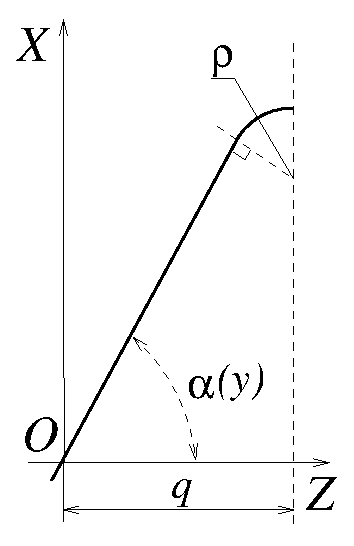
\includegraphics{qwave.eps}
\caption{$1/4\/$ of wave of the fan's neutral fibre. $O$ -- local origin of
coordinates, $q$ -- length of 1/4 of the fan's wave.}
\label{qwave}
\end{figure}


The description of the fan's geometry is based on a {\bf neutral
fibre}, defined as a wave-like three-dimensional surface in the middle
of the fan's thickness.

Fig.~\ref{qwave} represents the cross-section of the neutral fibre in the
plane parallel to the plane $OZX$ and displaced from the calorimeter axis
at a distance $y$. $1/4\/$ of a neutral fibre's wave is shown. 
It consists of a straight region, where $x = z \tan \alpha(y)$, and a fold
region. The fold radius $\rho$ does not depend on the distance to the
calorimeter axis.

\begin{figure}
\centering
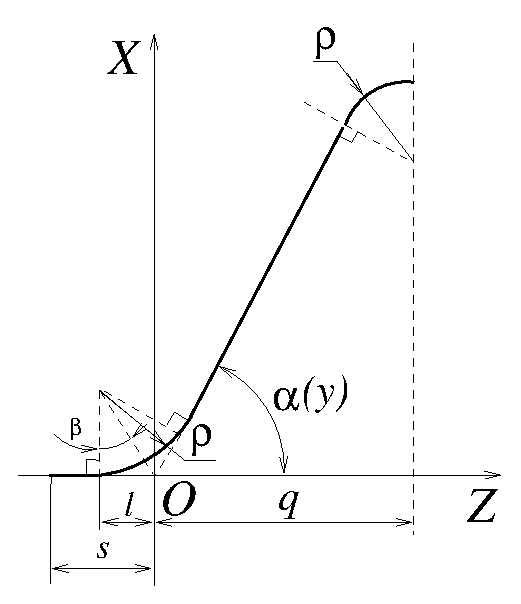
\includegraphics{bqwave.eps}
\caption{$1/4\/$ of the first wave of the fan's neutral fibre. $O$ -- local
origin of coordinates, $q$ -- length of 1/4 of the fan's wave.}
\label{bqwave}
\end{figure}


The geometry of first and last quarter-waves of a fan is a little different
(Fig.~\ref{bqwave}). The fold region that directly connects to the front or rear
wheel surface is of the same radius $\rho$ as a standard wave.
The flat part of the quarter-wave is directed to a point $s\/$ which
is a constant distance from the edge,
so the straight region ($s - l\/$) at the
beginning of the wave varies with $y\/$. The value of $l\/$ is given
by $\rho
\tan \beta\/$, where $\beta = \alpha / 2\/$.

All geometrical calculations in {\bf LArWheelSolid} are based on the
computation of the distance to a neutral fibre with the properties described
above.

\subsection{Practice}
A practical realization of a model of the geometry is based on the paper
\cite{geom_tables}, which  contains tables of neutral fibre sizes depending 
on the
distance to the calorimeter, and
the program \cite{simion}, where the fan wave slant angle $\alpha$ dependence
on the distance to the calorimeter axis is parameterized with a 4th-degree
polynomial.

Real absorbers and electrodes have a structure of several layers, with each
layer made of different materials. In {\bf LArWheelSolid} the multilayer
structure is replaced with a single-layer one using a ``mean'' material;
this is similar to the approach used in {\bf LArBarrelSolid}.

Some geometrical constants included in the code are given in Table~\ref{tg}.

\begin{table}[h]
\caption{Some geometrical parameters of the fan's neutral fibre.}
\label{tg}
\centering
\begin{tabular}{|p{0.4\textwidth}|c|c|}
\hline 
& inner wheel & outer wheel \\ \hline
number of waves in a fan  & 6 & 9 \\ \hline
wheel thickness (in the $Z$ direction) & \multicolumn{2}{c|}{514 mm} \\ \hline
starting and finishing fan-fold regions $s$ & \multicolumn{2}{c|}{2 mm} 
\\ \hline
fold radius $\rho$ & $3.25\/$ mm & $3.0\/$ mm \\ \hline
number of fans $n_{fan}$ in a wheel & 256 & 768 \\ \hline
%polar angle of a fan & $2\times0.055$ & $2\times0.015$ \\ \hline
absorber thickness (lead + steel + glue)& \shortstack{$(2.2 + 0.4 + 0.3)\/$\\
mm}& \shortstack{$(1.7 + 0.4 + 0.3)\/$ \\mm}\\ \hline
total thickness of an electrode &\multicolumn{2}{c|}{$275\/$ $\mu\/$m} \\ \hline
\end{tabular}\\
parameterization of the angle $\alpha(y) = a_0 + a_1y + a_2y^2 + a_3y^3 +
a_4y^4$\\ 
\begin{tabular}{|p{0.25\textwidth}|c|c|c|c|c|}
\hline
& $a_0$ & $a_1$ & $a_2\times10^3$ & $a_3\times10^7$ & $a_4\times10^{11}$  \\
\hline 
outer wheel & $-34.254$ & $0.15528$ & $-0.1167$ &
$0.45018$ & $-0.68473$\\ \hline
inner wheel & $-50.069$ & $0.50073$ & $-1.0127$ &
$10.39$ & $-42.176$\\ \hline
\end{tabular}
\end{table}

\section{Geant4 requirements}
In the Geant4 package a solid is a class; when you create a new type of solid
it must be inherited from the base class {\tt G4VSolid} and the following
methods must  be implemented \cite{G4VSolid}:
\begin{itemize}
\item {\tt Inside($\vec{p}\/$)} --- determines if the point $p$ 
is inside of solid, on its surface, or outside.
\item {\tt DistanceToIn($\vec{p}\/$), DistanceToOut($\vec{p}\/$)} 
--- determines the shortest distance from the point $p$ 
located outside or inside of the solid (respectively) to the solid surface.
\item {\tt SurfaceNormal($\vec{p}\/$)} --- 
determines a vector normal to the solid surface and going through the point
$p$. 
\item {\tt DistanceToIn$(\vec{p}, \vec{v})$}, 
{\tt DistanceToOut$(\vec{p}, \vec{v})$} --- compute the distance
from the point $p$ located outside or inside of the solid (respectively)
to the solid surface along the arbitrary vector $\vec{v}\/$.
\item {\tt GetEntityType}, {\tt DescribeYourselfTo}, {\tt GetExtent},
{\tt CreatePolyhedron}, 
{\tt CreateNURBS} --- special functions for tracking and solid drawing.
\end{itemize}

One important thing which I encountered is the following: the information
given by the functions mentioned above must be self-consistent. For
example, if {\tt DistanceToIn$(\vec{p}, \vec{v})$} returns value $d$ then
{\tt Inside($\vec{p} + d |\vec{v}|)$} should not return ``outside''. Otherwise
the Geant4 tracking algorithm may enter into an infinite loop on the solid surface.

\section{Algorithms and data of {\tt LArWheelSolid}}
\begin{table}
\caption{Data of {\tt LArWheelSolid}}
\label{data}
\centering
\begin{tabular}{|p{0.5\textwidth}|p{0.5\textwidth}|}
\hline
{\tt LArWheel\_t Type} & wheel type (see subsection \ref{type})\\ \hline
{\tt G4double FanHalfThickness} & half of a fan thickness\\ \hline
{\tt static const G4double WheelThickness} & wheel thickness (along $Z$ axis)\\
\hline 
{\tt static const G4double StraightStartSection} & size of starting and
ending fan fold regions ($s$)\\ \hline
{\tt G4double quarterWaveLength} & quarter of a fan wave length \\ \hline 
{\tt G4double HalfWaveLength} & half of a fan wave length \\ \hline
{\tt G4double FanFoldRadius} & fold radius ($\rho$)\\ \hline
{\tt G4int NumberOfWaves} & number of waves in a fan\\ \hline
{\tt G4int NumberOfHalfWaves} & {\tt NumberOfWaves}$ / 2$\\ \hline
{\tt G4int NumberOfFans} & number of fans in the wheel ($n_{fan}$) \\
\hline 
{\tt G4double ZeroFanPhi} & polar angle of fan number zero\\ \hline
{\tt G4double ZeroFanPhi\_ForDetNeaFan} & see subsection \ref{det_nea_fan} \\ \hline
{\tt G4double FanStepOnPhi} & step in $\phi$ between fans
($2\pi / n_{fan}$)\\ \hline
{\tt FanPhiAmplitude} & polar angle half-size of a fan \\ \hline
{\tt static const G4double Tolerance} & precision of solid boundary
determination  \\ \hline
{\tt static const G4double IterationPrecision } & precision required to stop
iteration calculation\\ \hline
{\tt static const G4double IterationPrecision2} & second power of
{\tt IterationPrecision }\\ \hline 
{\tt static const unsigned int IterationsLimit} & maximal number of iterations;
required for loop breaking in case of error\\ 
\hline 
{\tt G4Polycone *BoundingPolycone} & see subsection \ref{bpcone}\\ \hline
{\tt G4Polycone **FanSection} & see subsection \ref{fan_sect}\\ \hline
\shortstack[l]{\tt G4double\\ (*parameterized\_slant\_angle)()} & see subsection
\ref{par_sla_ang} \\ \hline
{\tt static LArWheelSolid* m\_static\_inner\_wheel} &  \\
{\tt static LArWheelSolid* m\_static\_inner\_wheel} & see subsection
\ref{static_wheel}\\ 
{\tt G4int (*get\_phi\_gap)()} & \\ \hline
\end{tabular}
\end{table}

Due to the calorimeter's axial symmetry, all the input parameters are
translated to the coordinate system where the fan is positioned along
the $OY\/$ axis. All further calculations are conducted in the
coordinate system relative to this {\bf ``vertical''} fan. If it is
necessary, after the calculation the results are translated back into
the initial coordinate system.

It is recommended that the {\tt LArWheelSolid} code (files {\tt
LArWheelSolid*} in the {\tt src} and {\tt LArG4EC} subdirectories) be
consulted while reading this paper.

In Table~\ref{data} each important data element is listed 
with a short comment about
its purpose. 
Some data members are not listed in the table; they are described separately.

Please note that, unlike older versions, the absorber and electrode
solids cannot be used independently. Many of the {\tt LArWheelSolid} algorithms now 
rely on the fact that there
is an electrode between each two absorbers and vice versa. This approach is used
because it significantly improves performance.

\subsection{\tt LArWheel\_t}\label{type}
{\tt LArWheel\_t} --- special enumerator type.
Variables of this type can be one of four values: {\tt InnerAbsorberWheel},
{\tt InnerElectrodWheel}, {\tt OuterAbsorberWheel},\\ {\tt OuterElectrodWheel}.
The {\tt LArWheelSolid} constructor takes a parameter of this type; 
it indicates which type of wheel is being defined: 
inner or outer, absorber or electrode.
It is assumed that physical volumes made of each type of wheel will be positioned
at a common place (at the vector $(0, 0, Z_0)$). If so, the relative positions 
will be correct: electrodes between absorbers of the corresponding wheel,
the outer wheel surrounds the inner one.

\subsection{\tt distance\_to\_neutral\_fibre$(\vec{p})$}
This is the most important function.
It returns the shortest distance from the point $p$ to the neutral fibre of the
vertical fan. The returned value is positive if $p$ is positioned in
the region of relatively greater polar angle to the neutral fibre, and negative
otherwise.

The function uses an approximation: for 
the calculation of the angle $\alpha(y)$ $y\/$-coordinate of $p$ is used instead
of correct value of $y$-coordinate
 in the point of the neutral fibre nearest to $p$. 
The calculations are made in the plane parallel to plane $OZX$ and going through
the point $p$. The routine makes use of the symmetry of waves of the 
neutral fibre about the ``knot'' (the point of inflection at $O$ in
Fig.~\ref{qwave}).

Using $p_z$ the function determines the quarter-wave of the
neutral fibre nearest to $p$. If this is neither the first nor the last quarter-wave, the 
coordinates $(p_z, p_x)$ are transformed in the following way:
\begin{enumerate}
\item  a shift on $z$ is performed, so the local coordinate origin
$O$ is moved to the knot point,
\item odd half-waves are mirrored relatively to local $OZ$ axis,
\item odd quarter-waves are additionally inverted relative to
local coordinate origin $O$.
\end{enumerate}

After these transformations, all the initial cases are moved into a
standard coordinate system: the nearest quarter-wave where
local coordinates $z$ and $x$ are positive (Fig.~\ref{qwave}).

\begin{figure}
\centering
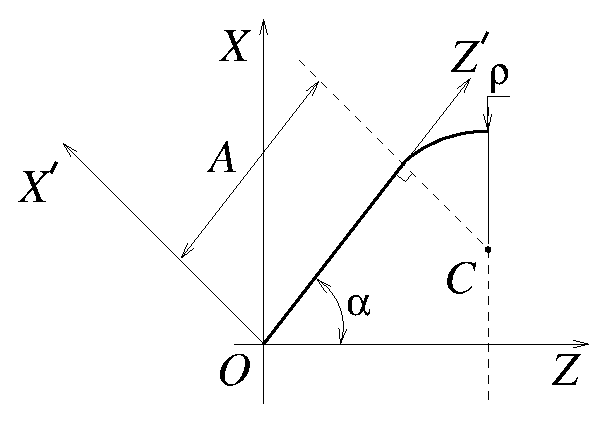
\includegraphics{qwave_prime.eps}
\caption{Calculation of distance $d$ from point $(z, x)$ to neutral fibre. 
If $z^{\prime}< A\/$, then  $d=x^{\prime}\/$, else $d =
\sqrt{(x^{\prime}-A)^2 + (z^{\prime}+\rho)^2} - \rho\/$.}
\label{qwave_prime}
\end{figure}


Next, the local coordinate system is rotated so the straight part of the quarter-wave
is positioned along the $Z^{\prime}$ axis (Fig.~\ref{qwave_prime}).
In this coordinate system it is easy to determine if the initial point is
nearer to
the straight part of the quarter-wave or to the fold region. In both cases the
distance is computed using simple exact two-dimensional formulae.

At the end the result is given with the correct sign, depending on
which transformations were performed.

\begin{figure}
\centering
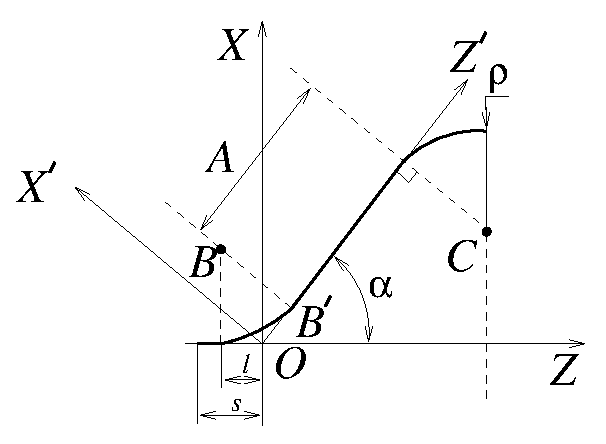
\includegraphics{bqwave_prime.eps}
\caption{Calculation of the distance $d$ from point $(z, x)$ to the
fan's neutral fibre, in the case of the starting quarter-wave.
If $z < -l\/$ and the input point is below the $BB^{\prime}\/$ line, then $d = x$.
If $z^{\prime} < l\/$, then $d =
\sqrt{(x^{\prime}-\rho)^2 + (z^{\prime}-l)^2} - 
\rho\/$, if $z^{\prime}< A\/$, then  $d=x^{\prime}\/$,
else $d = \sqrt{(x^{\prime} + \rho)^2 +
(z^{\prime}-(A + l))^2} - \rho\/$. } 
\label{bqwave_prime}
\end{figure}


In the case of first and last quarter-waves the situation becomes more complex
due to
the existence of the additional fold region.
Using symmetry the last quarter-wave is transformed to the first one.
The next steps are almost the same as the ones for the regular quarter-wave;
the only
exception is that the local coordinate origin is positioned while transforming, not
into
the beginning of the quarter-wave, but into the cross point of the straight part
that continues into the local $OZ$ axis (Fig.~\ref{bqwave_prime}). 

According to measurements, the error of the
distance to the neutral fibre determined by this technique is not more
 than several tens of
microns. This is sufficient for most applications.

\subsection{\tt nearest\_point\_on\_neutral\_fibre$(\vec{p})$}
This function is nearly identical to the function {\tt
distance\_to\_neutral\_fibre}
and uses the same approximation technique.
 The function returns the point on the
vertical fan neutral fibre which is the ``nearest'' to $p$ as defined by {\tt
distance\_to\_neutral\_fibre}.

\subsection{\tt determine\_nearest\_fan$(\vec{p})$}\label{det_nea_fan}
The function determines the fan nearest to the given point.
It searches for a pair of fans of {\em different from the current solid} type
containing the point between them using the following algorithm.
First of all, using the formula
\[i = \mbox{int}((p_{\phi} - \pi/2 - {\tt ZeroFanPhi\_ForDetNeaFan}) /
{\tt FanStepOnPhi})\] 
the number of one of the nearest-to-the-point fans is determined. {\tt
ZeroFanPhi\_ForDetNeaFan} is {\tt ZeroFanPhi} for the different type of wheel.
Next, the neighboring fans are checked one by one until the fan's pair will be
found, the distance from $p$ to the neutral fibre of the first fan of the pair
is positive and the distance to the second one is negative.
That means that $p$ is located between the fans of this pair. There is a fan of
current type between them which is the nearest one to the point $\vec{p}$.

\subsection{\tt distance\_to\_nearest\_fan$(\vec{p})$}
This method acts
 like the {\tt determine\_nearest\_fan}, but returns distance to the nearest
fan's neutral fibre. Vector $\vec{p}$ is modified.

\subsection{\tt BoundingPolycone}\label{bpcone}
{\tt BoundingPolycone} is an object of class {\tt G4Polycone}, which represents 
a wheel surface. It helps to easily process points which are outside the wheel's
boundaries.

The {\tt BoundingPolycone} is also used to represent the solid for 
some Geant4 special functions.

Now {\tt BoundingPolycone} is constructor parameter although I don't like such
approach.
{\tt BoundingPolycone} is initialized in {\tt LArEMECConstrucion.cc}.

\subsection{\tt Inside$(\vec{p})$}
This function checks if the point $p$ is inside of the {\tt BoundingPolycone}. If
it is, then it determines the distance to the nearest-to-$p$ fan and 
checks if the
point is inside or on the surface (comparing the distance with {\tt
HalfFanThickness}).

\subsection{\tt DistanceToIn$(\vec{p})$}
The function checks if the point $p$ is not outside of the {\tt
BoundingPolycone}. If yes, then it determines the distance to the nearest-to-$p$
fan's neutral fibre and subtracts {\tt HalfFanThickness}. Otherwise it 
pases $p$ to the {\tt DistanceToIn$(\vec{p})$} method of {\tt BoundingPolycone}. 

\subsection{\tt DistanceToOut$(\vec{p})$}
The function checks if the point $p$ is not outside of the {\tt
BoundingPolycone}. If 
yes, then it determines the distance to the nearest fan's neutral fibre,
calculates the distance to the fan's surface, compares it with the distance to
the {\tt BoundingPolycone}'s surface and returns the smaller one. If the point
is not inside of the fan or it is outside of the {\tt BoundingPolycone} the
function returns zero.

\subsection{\tt SurfaceNormal$(\vec{p})$}
The function checks if the point $p$ is inside the {\tt BoundingPolycone}. If
yes, then it determines the nearest fan, finds the nearest point on the fan's
neutral fibre and returns the unit vector pointing to $p$ from this point.
Otherwise it 
passes $p$ to the {\tt SurfaceNormal$(\vec{p})$} method of {\tt BoundingPolycone}.

\subsection{\tt FanSection}\label{fan_sect}
The array {\tt FanSection} contains objects of type {\tt G4Polycone} each of
which corresponds to sections of the vertical fan.
{\tt FanSection[i]} is a polyconical sector containing the whole 
half-wave of the vertical fan. First and last half-waves have two fan sections,
for the starting/finishing fold region and the nearby quarter-wave separately.
$Z$-boundaries of fan sections 
are stored in the array {\tt FanSectionLimits}. Data members
{\tt MaxFanSection} and {\tt MaxFanSectionLimits} contain the maximum (for a given
wheel type) numbers of fan sections and their edges correspondently.

The polar angle size of a fan section is enough to capture all the points 
between the vertical fan and its nearest neighbors.

The {\tt FanSection[i]} objects are used by the functions that calculate the
distance to the solid surface along an arbitrary vector.

The initialization of the {\tt FanSection} array is made by function \\
{\tt inner\_wheel\_init} or {\tt outer\_wheel\_init}.

\subsection{\tt out\_iteration\_process$(\vec{p}, \vec{q})$}
This function searches for the exit point of segment $pq$ from the fan's
half-wave in the event that $q$ is not inside the fan. The points $p$ and $q$
should be in the same {\tt FanSection}.

The function uses an iterative technique of dividing a segment in half.
At the $i\/$th step 
\[\vec{p}_{i+1} = \frac{\vec{p}_i+\vec{q}_i}{2}, \vec{q}_{i+1} = \vec{q}_i,\]
if the point $\frac{\vec{p}_i+\vec{q}_i}{2}$ is not outside the fan, and
\[\vec{p}_{i+1} = \vec{p}_i,  \vec{q}_{i+1} = \frac{\vec{p}_i+\vec{q}_i}{2},\]
otherwise. The process stops when
$|\vec{p}_i-\vec{q}_i|<{\tt IterationPrecision\/}\/$ or $i$ has reached the {\tt
IterationsLimit}.

\begin{figure}
\centering
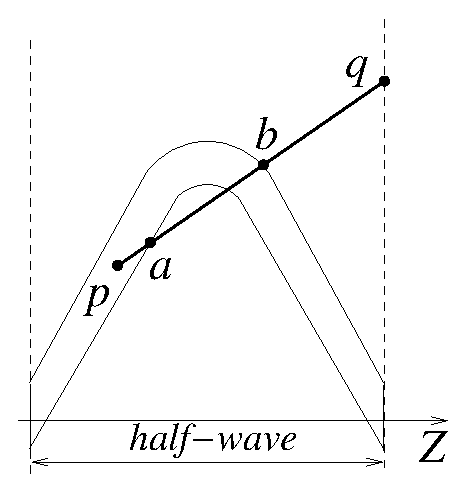
\includegraphics[width=0.33\textwidth,height=0.4\textwidth]{out_iter.eps}
\caption{}
\label{out_iter}
\end{figure}

When a situation is like that shown in Fig.~\ref{out_iter}, 
the function may either find point $a$ or point $b$. It is up to the user to
spot the potential ambiguity and call this function again.

The function returns the distance from the point $p$ to one of the exiting
points. The exiting point is not inside the fan.
 
\subsection{\tt search\_for\_most\_remoted\_point$(\vec{p}, \vec{q}, \vec{r})$}
This function searches on the segment $pq$ for the point which is the
most distant from the neutral fibre of the vertical fan and sets
vector $r$ to it. It also returns a boolean value which is true if
during the search a point outside the vertical fan is encountered
(this allows us to apply {\tt out\_iteration\_process$(\vec{p},
\vec{r})$} here) or false if $pq$ is completely inside the vertical
fan (in this case $r$ is useless). The points $p$ and $q$ should be in
the same {\tt FanSection}.

Next there is a search for the most distant point of segment
$pq$ from the neutral fibre. The search is performed by successively 
dividing the segment in half and looking for the point
where second power of the distance $d$
from segment $pq$ to the neutral fibre is maximal.
At the $i\/$th step 
\[ \vec{p}_{i+1} = \frac{\vec{p}_i+\vec{q}_i}{2}, \vec{q}_{i+1} = \vec{q}_i,\]
if the sign of the derivative $(d^2)^{\prime}$ in the point
$\frac{\vec{p}_i+\vec{q}_i}{2}$ is positive and 
\[\vec{p}_{i+1} = \vec{p}_i, \vec{q}_{i+1} = \frac{\vec{p}_i+\vec{q}_i}{2},\]
otherwise. 
The sign of $(d^2)^{\prime}$ is defined as the sign of the expression
\[d^2(\frac{\vec{p}_i+\vec{q}_i}{2}) -
d^2(\frac{\vec{p}_i+\vec{q}_i}{2}-\vec{\delta})\/,\] where \[\vec{\delta} =
\frac{\vec{q}-\vec{p}}{|\vec{q}-\vec{p}|}\times{\tt IterationPrecision}\] is
small vector along the segment $pq$. 
The process is stopped when 
$|\vec{p}_i-\vec{q}_i|<{\tt IterationPrecision}$ or $i$ has reached the {\tt
IterationsLimit\/}. The process is stopped prematurely if the point
$\frac{\vec{p}_i+\vec{q}_i}{2}$ is situated outside of the fan.

If the process has not been stopped prematurely that means the whole segment
$pq$ is inside the current half-wave of the fan.

\subsection{\tt distance\_to\_out$(\vec{p}, \vec{v})$}
This function calculates the distance along the vector
$\vec{v}$ from the point $p$ to the surface of the vertical fan. $\vec{v}$
should be a unit vector. 

First, the function determines in which {\tt FanSection} the point $p$
is located and finds point $a$, the exit point of the line
$\vec{p}+\vec{v}t$ out of the {\tt FanSection}. 
If $a$ is outside of the vertical fan then the function\\ 
{\tt out\_iteration\_process} is called and the line's exit point $q$ out of
the fan is found. Due tothe  potential ambiguity 
of the {\tt out\_iteration\_process} result, it is
not safe to assume that the point $q$ is the nearest exit point.
If the point $a$
is positioned inside the fan then $q$ is set equal to $a$.

Next there is a search for the most distant point of segment
$pq$ from the neutral fibre.
If there is a point outside the vertical fan on $pq$, then a
new {\tt out\_iteration\_process} is called and its result is returned.

If the point $q$ has been found
earlier by the function {\tt out\_iteration\_process} then $q$ is the point
desired, and the function returns the length of the segment $pq$. Otherwise the
search for the exit point is performed in the neighbor half-wave of the fan
in the direction of the segment $pq$.
The search transition is not performed if $pq$ is directed beyond the beginning of the
first half-wave or beyond the end of last half-wave of the fan. In that case the
function returns the length of the segment $pq$.

Due to the properties of the geometry the search for the exiting point in the
neighbor half-wave could sometimes be simplified.

\subsection{\tt DistanceToOut$(\vec{p}, \vec{v}, \dots)$}
This function checks if the point $p$ is inside of the {\tt BoundingPolycone}. If
yes, then it determines inside of which fan the point $p$ is positioned and
returns the distance to the fan's surface along the vector $\vec{v}$. If the
point $p$ is not inside of any fan or outside of the
{\tt BoundingPolycone}, zero is returned.

The function has three more parameters, which are substituted by ``\dots'' in
the header. These parameters are {\tt G4bool calcNorm}, {\tt G4bool *ValidNorm}
and {\tt G4ThreeVector *n}. According to Geant4 rules, if the {\tt calcNorm} is
true then the function has to set parameters {\tt *ValidNorm} and
{\tt *n} in a defined way. {\tt DistanceToOut} always sets the {\tt *ValidNorm} to false. That
means the solid does not lie entirely behind the exiting surface\footnote{This
is not absolutely correct, but is not of great importance. Probably I'll correct
it in the future.}.
The value of {\tt *n} has no meaning in this case.

\subsection{\tt in\_iteration\_process$(\vec{p}, \vec{q})$}
This function searches the entrance point of segment $pq$ into the vertical
fan when points $p$ and $q$ are positioned on different
sides of the neutral fibre. (This means that the distances from $p$ and from $q$ to
the neutral fibre are of the different signs.) 

The function uses the iterative technique of dividing a segment in half. At the
$i\/$th step
\[\vec{p}_{i+1} = \vec{p}_i,  \vec{q}_{i+1} = \frac{\vec{p}_i+\vec{q}_i}{2},\]
if the point $\frac{\vec{p}_i+\vec{q}_i}{2}$ is positioned on a different
side of the neutral fibre from point $p$ or is not located outside of the 
fan, and
\[\vec{p}_{i+1} = \frac{\vec{p}_i+\vec{q}_i}{2}, \vec{q}_{i+1} = \vec{q}_i,\]
otherwise. The process stops when
$|\vec{p}_i-\vec{q}_i|<{\tt IterationPrecision\/}\/$ or $i$ has reached the {\tt
IterationsLimit\/}.

The function returns the distance from the point $p$ to the entrance
of segment $pq$ into the fan. The resulting point is not outside the fan.

The function also requires as a parameter the distance from point $p$ to the
neutral fibre. Usually this value has already been calculated somewhere in a
calling routine, so it helps to exclude unnecessary calculations.

\subsection{\tt search\_for\_nearest\_point$(\vec{p}, \vec{q})$}
This function searches for the point on the segment $pq$ for which the
 distance $d$ to the neutral fibre of the vertical fan is minimal. It
 is assumed that value of $d$ is unique.  The points $p$ and $q$ are
 positioned on the same side of the neutral fibre, so the signs of
 $d(\vec{p})$ and $d(\vec{q})$ are equal. If they are negative it is
 taken into account by the corresponding way: {\tt kInfinity} is returned
 if the point of segment $pq$ nearest to the neutral fibre is outside
 of the fan; if the point is inside the fan the value returned is the
 distance from $p$ to the fan's surface along the segment $pq$.

The search is conducted by dividing the segment in half.
At the $i\/$th step 
\[ \vec{p}_{i+1} = \frac{\vec{p}_i+\vec{q}_i}{2}, \vec{q}_{i+1} = \vec{q}_i,\]
if the sign of the derivative $d^{\prime}$ in the point
$\frac{\vec{p}_i+\vec{q}_i}{2}$ is negative, and \[\vec{p}_{i+1} = \vec{p}_i,
\vec{q}_{i+1} = \frac{\vec{p}_i+\vec{q}_i}{2},\] 
otherwise. 
The sign of $d^{\prime}$ is defined as the sign of the expression
\[d(\frac{\vec{p}_i+\vec{q}_i}{2}) -
d(\frac{\vec{p}_i+\vec{q}_i}{2}-\vec{\delta})\/,\] where \[\vec{\delta} =
\frac{\vec{q}-\vec{p}}{|\vec{q}-\vec{p}|}\times{\tt
  IterationPrecision}\] is a
small vector along the segment $pq$. 
The process is stopped when
$|\vec{p}_i-\vec{q}_i|<{\tt IterationPrecision}\/$ or $i$ has reached the {\tt
IterationsLimit}. The process is stopped prematurely if 
the point $\frac{\vec{p}_i+\vec{q}_i}{2}$ is located on the opposite side
of the neutral fibre from point $p$. In this case function \\
{\tt in\_iteration\_process$(\vec{p}, \frac{\vec{p}_i+\vec{q}_i}{2})$} is called
and the result is returned. 

If the process has not been stopped prematurely and the resulting
 point is inside of the fan then the
function {\tt in\_iteration\_process} is called, and its result is returned.
Otherwise, the function checks if $p$ or $q$ are inside, and, if yes, selects the
nearest to the neutral fibre; if not,
the whole segment $pq$ is outside the fan and the
function returns {\tt kInfinity}.

The resulting point is not outside the fan.

\subsection{\tt distance\_to\_in$(\vec{p}, \vec{v})$}
This function calculates the distance from the point $p$ to the vertical fan's
surface along the vector $\vec{v}$.

First, a {\tt FanSection} containing point $p$ is selected. The point $q$ is
found, where $q$ is intersection of the line $\vec{p}+\vec{v}t$ 
with the surface of the current {\tt FanSection}. If the points $p$
and $q$ are positioned on the different sides of the fan's neutral fibre
then the intersection of $\vec{p}+\vec{v}t$
and the fan is certainly between the
boundaries of the current half-wave; the function {\tt
in\_iteration\_process$(\vec{p}, \vec{q})$} is called, and its result is
returned. Otherwise the function {\tt search\_for\_nearest\_point$(\vec{p},
\vec{q})$} is called. If its result is {\tt kInfinity}
then there is no intersection
in the current half-wave; otherwise the result is the distance desired and the
function returns it.

If there is no intersection with the current half-wave, then the search is moved
to the neighboring half-wave along the direction of the vector $\vec{v}$. If
$\vec{v}$ points beyond the beginning of the first half-wave or beyond the end of
the last half-wave, search is not moved and the function returns {\tt kInfinity}.

If the result is still not obtained, it is necessary to search for entrance
point
in the two neighboring fan sections in the 
direction of $\vec{v}$; any other sections are hidden by
the neighboring fans.

\subsection{\tt DistanceToIn$(\vec{p}, \vec{v})$}
The function checks if the point $p$ is inside of the {\tt BoundingPolycone}.
If it is outside, the function tries to find out the entrance point into the {\tt
BoundingPolycone}, calculates distance from that point to the nearest fan and
returns the sum of these two distances.
If $p$ is inside, the function just determines the distance required.

\subsection{\tt parameterized\_slant\_angle}\label{par_sla_ang}
This data member is initialized as a pointer to one of the\\ {\tt
parameterized\_slant\_angle\_inner()} or\\ {\tt
parameterized\_slant\_angle\_outer()}
methods. These methods calculate wave slant angle $(\alpha(y))$ for
the inner and
outer wheels respectively.

\subsection{\tt GetPhiGap$(${\em wheel type}$, \vec{p})$}\label{static_wheel}
There are two static data members in the class. {\tt m\_static\_inner\_wheel}
and {\tt m\_static\_outer\_wheel} are initialized by the class constructor with
pointers to one of electrode wheels of corresponding type. These pointers are
used by {\tt get\_phi\_gap\_wheel} to find out between which electrodes the
point $p$ is ({\tt determine\_nearest\_fan} is used). The point should be in
local coordinate system. Public static method {\tt GetPhiGap} is
available. The
{\tt get\_phi\_gap} method is defined in the class {\tt LArWheelModuleSolid} (sec. \ref{lwms}).

\subsection{\tt GetGapSize$(${\em wheel type}$, \vec{p})$}
This static public function calculates liquid-argon gap size for the point $p$
in the given wheel. It also uses {\tt m\_static\_inner\_wheel} and {\tt
m\_static\_outer\_wheel} and follows an algorithm similar to one used in {\tt
determine\_nearest\_fan}.

\section{LArWheelModuleSolid}\label{lwms}
This solid is a descendant of {\tt LArWheelSolid}. Its purpose is to
describe a
separate EMEC module for test-beam simulations. It mostly uses conventional {\tt
LArWheelSolid} methods but overloads some to correctly account for some tracking
effects on phi module edges.

The main differences are:
\begin{itemize}
\item {\tt BoundingPolycone} for this solid is a polyconical sector. It is
created from a polycone passed as constructor parameter.
\item All methods check if the fan determined as nearest really exists. If not,
they take second-nearest one.
\item In {\tt DistanceToIn$\vec{p}, \vec{v})$} when processing first or last
absorber fan: if the entrance point is not found in
current {\tt FanSection}, then search in all other sections, not only in 
the neighboring fan.
\end{itemize}

\section{LArFanSolid}
There was an attempt to create a Geant4 solid for a separate fan. {\tt
LArFanSolid}'s algorithms are the same as for the vertical fan of {\tt
LArWheelSolid}, while transformation to the fan's local coordinate system is
left for Geant4 standard tracking.

The reasons for creating such solid were:
\begin{enumerate}
\item I expected a performance improvement compared with the conventional approach,
\item it looks like it would be easier to describe an individual fan's deformation,
\item it is easier to create a separate module description for test-beam (and,
actually, such an approach would be more reliable),
\item and there were some minor useful things.
\end{enumerate}

Unfortunately, the first version of {\tt LArFanSolid} is very slow. So
for now, the
development of this branch is frozen. I think we may spare some time for speed
investigations of this solid in the future. Maybe we will need to work with {\tt
LArFanSolid} to implement deformations.

\section{Visualisation}
I can hardly imagine how to visualize such a complex solid like {\tt
LArWheelSolid} using conventional Geant4 tools. So for Geant4 visualization the
solid's objects look like their corresponding bounding polycones. But it is very
useful to be able to draw the detailed structure of fans. A special
program has been written for this purpose. It allows one to draw any cross-section of any
EMEC wheel and to test all the mandatory G4Solid methods of {\tt
LArWheelSolid}. For  details the reader is referred to the file
LArG4/doc/README.EMECVis in the LArG4 package.

\section{Notes on future development}
It is necessary to integrate {\tt LArWheelSolid} and {\tt LArWheelCalculator},
as suggested in the LArG4 Application Guide. There is also some room for speed
improvements. Further investigations on {\tt LArFanSolid} are warranted.

\begin{thebibliography}{10}
\bibitem{G4} \underline{\em http://wwwinfo.cern.ch/asd/geant4/} --- Geant4
Homepage.
\bibitem{EMEC} ATLAS Technical Design Report, Ch. 7 --- {\em ``The
electromagnetic end-cap calorimeter and presampler''\/}.
\bibitem{r1} A. Chekhtman, D. Fouchez, E. Monnier. {\em ``The Accordion in the
end-cap: geometry and characteristics''\/}, ATALS-LARG-NO-4.
\bibitem{r2} S. Klimenko, Yu. Tikhonov, A. Chekhtman. {\em ``The Design of
Endcap EM Calorimeter with Constant Thickness of the Absorber Plates''\/},
ATLAS-LARG-NO-025.
\bibitem{r3} O. Martin, E. Monnier, S. Tisserant. {\em ``Update of some
Geometrical Parameters for the ATLAS E.M. End-Cap Calorimeter''\/},
ATALS-LARG-NO-047. 
\bibitem{geom_tables} L. Martin, J.-L. Gimenez, A. Chekhtman. {\em ``Creating
IGES files of absorbers''} (ABS.YYY.00.DRa.3).
\bibitem{simion} Programme {\tt white\_may2000.f} written by S. Simion.
\bibitem{G4VSolid} Geant4 User's Guide --- For Toolkit Developers, sec. 4
``Geometry''.
\end{thebibliography}

\end{document}
